\label{chap:ann}
In this chapter we will make an overview about neural networks and some other concepts for a reader better comprehension of the following parts of the thesis.

\section{Introduction}
The Artificial Neural Networks is a family of classification technique\footnote{Classification is the operation of learning a function \textbf{$f$} that map example records \textbf{$x \in D$}, where $D$ is the set of \textbf{$(x, y)$}, to the labels set \textbf{$y$} (the classes). This target function is called also Classification Model and is used in a descriptive or predictive way problem depending.}, that are inspired by the human brain: in particular by the connections inside this latter. The human brain consists principally of nerve cells called \textbf{neurons}, that are connected together via the \textbf{axons} used to transmit the electrical impulse by a neuron to another. This electrical impulse generated by a stimulated neuron is transferred to another one via the dendrites, a particular elements in the human brain used to connect two neuron: this point of contact is called synapse. \newline\newline
Analogously the internal structure of a Neural Network is composed by components called \textbf{neurons}, connected together by directed links. There are many types of Neural Networks, but for the sake of simplicity and  for the scope of the thesis we will focus the attention to feedforward neural network model, explaining firstly the Perceptron model.

\section{Perceptron}\label{sec:perceptron}
The Perceptron model is the basic and simplest type of Neural Network, proposed firstly in \cite{ROSE:1958}. This model is composed only by two types of nodes called \textbf{input nodes} and \textbf{output node}. As we can see in the Figure \ref{fig:illustration-perceptron-model}, the input nodes and the output node are connected by weighted links similarly to the human brain, that are used to simulate the synaptic connections strength.\newline\newline
\begin{figure}[t]
	\centering

	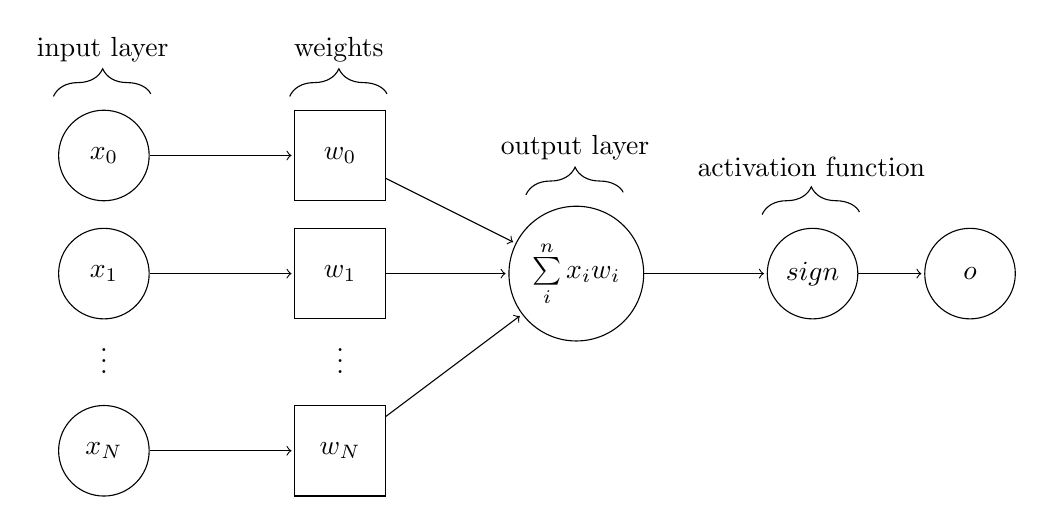
\begin{tikzpicture}[shorten >=1pt]
		\tikzstyle{unit}=[draw,shape=circle,minimum size=1.15cm]
		%\tikzstyle{hidden}=[draw,shape=circle,fill=black!25,minimum size=1.15cm]
		\tikzstyle{hidden}=[draw,shape=circle,minimum size=1.15cm]
		\tikzstyle{weights}=[draw,shape=rectangle,minimum size=1.15cm]

		\node[unit](x0) at (0,3.5){$x_0$};
		\node[unit](x1) at (0,2){$x_1$};
		\node at (0,1){\vdots};
		\node[unit](xd) at (0,-0.25){$x_N$};

		\node[weights](w0) at (3,3.5){$w_0$};
		\node[weights](w1) at (3,2){$w_1$};
		\node at (3,1){\vdots};
		\node[weights](wd) at (3,-0.25){$w_N$};

		\node[unit](y1) at (6, 2){$\sum\limits_{i}^{n}{x_iw_i}$};

		\node[unit](f) at (9, 2){$sign$};
		
		\node[unit](o) at (11, 2){$o$};

		\draw[->] (x0) -- (w0);
		\draw[->] (x1) -- (w1);
		\draw[->] (xd) -- (wd);
		
		\draw[->] (w0) -- (y1);
		\draw[->] (w1) -- (y1);
		\draw[->] (wd) -- (y1);

		\draw[->] (y1) -- (f);
		
		\draw[->] (f) -- (o);
			
		\draw [decorate,decoration={brace,amplitude=10pt},xshift=-4pt,yshift=0pt] (-0.5,4.25) -- (0.75,4.25) node [black,midway,yshift=+0.6cm]{input layer};
		\draw [decorate,decoration={brace,amplitude=10pt},xshift=-4pt,yshift=0pt] (2.5,4.25) -- (3.75,4.25) node [black,midway,yshift=+0.6cm]{weights};
		\draw [decorate,decoration={brace,amplitude=10pt},xshift=-4pt,yshift=0pt] (5.5, 3) -- (6.75, 3) node [black,midway,yshift=+0.6cm]{output layer};
		\draw [decorate,decoration={brace,amplitude=10pt},xshift=-4pt,yshift=0pt] (8.5, 2.75) -- (9.75, 2.75) node [black,midway,yshift=+0.6cm]{activation function};
	\end{tikzpicture}
	\caption{Perceptron model illustration}\label{fig:illustration-perceptron-model}
\end{figure}	
This model calculates the output $\hat{y}$ as a weighted sum of the input with respect to the connections weight, to which is summed the bias (a value used to rectify, in this case, the neural network output). So recalling some math, the output of the Perceptron model can be expressed in the following way:
\begin{equation}
	\hat{y} = \textbf{g}(w_{0}x_{0} + w_{1}x_{1} + \dots + w_{N}x_{N} + b  ) = \textbf{g}(\textbf{w} \bullet \textbf{x} + \textbf{b})
\end{equation}
where $i = 1, \dots, N$ and $N$ is the cardinality of the vector $\textbf{x}$ and the $\textbf{g}$ acts as the activation function.
The training of the Perceptron consists in recompute (the key passage at the step 7 of Algorithm \ref{alg:perceptron-learning}), or more precisely update, in an iterative manner the connections weight until they are able to fit the input data, i.e. the examples $(x, y) \in D$, optimizing the objective function.
At the step 7 of the Algorithm \ref{alg:perceptron-learning}
\begin{center}
	$w_{j}^{(k + 1)} = w_{j}^{(k)} + \lambda(y_{i} + \hat{y}_{i}^{(k)})x_{ij}$	
\end{center}
where $w_{j}^{(k)}$ is the connection weight at the step $k$, $\lambda$ is the learning rate\footnote{Learning rate is a parameter that indicates to the optimization algorithm how much quickly the neural network must abandons the "old beliefs" substituting them with the new ones, or in other words, how much the connections weight are updated.} and $x_{ij}$ is the $j^{th}$ feature of the $i^{th}$ example.

\begin{algorithm}
	\begin{algorithmic}[1]
		\State{Let $D = \{(\textbf{x}_i, y_i)\ |\ i  = 1, \dots, N\}$ be the set of examples.}
		\State{Initialize the weight vector with random values, $\textbf{w}^{(0)}$}
		\Repeat
			\For{ each example $(\textbf{x}_{i}, y_{i}) \in D$}
				\State Compute the predicted output $\hat{y}_{i}^{(k)}$
				\For{ each weight $w_i$}
					\State Update the weight $w_{j}^{(k + 1)} = w_{j}^{(k)} + \lambda(y_{i} + \hat{y}_{i}^{(k)})x_{ij}$
				\EndFor
			\EndFor
		\Until{ Stopping condition is met }
	\end{algorithmic}
	\caption{Perceptron learning algorithm \cite{ITDM:2014}}\label{alg:perceptron-learning}
\end{algorithm}

\section{Multi-Layer Perceptron (MLP)}
The Multi-Layer Perceptron (MLP), known as feedforward neural network, is been created principally to resolve the problems of the Perceptron because:
\begin{itemize}
	\item{It cannot handles a domain $(\textbf{x}, y) \in D$ with more than two classes, because it divides the input data in only two boundaries, as it can be seen in the figure \ref{fig:perceptron-boundaries}, so more dimensions can not be handled}
	\item{It can not converge if the data is not linearly separable and this leads to reduce the use of Perceptron in many few case (trivially, when the data is linearly separable)}
\end{itemize}

\begin{figure}[t!]
	\centering
	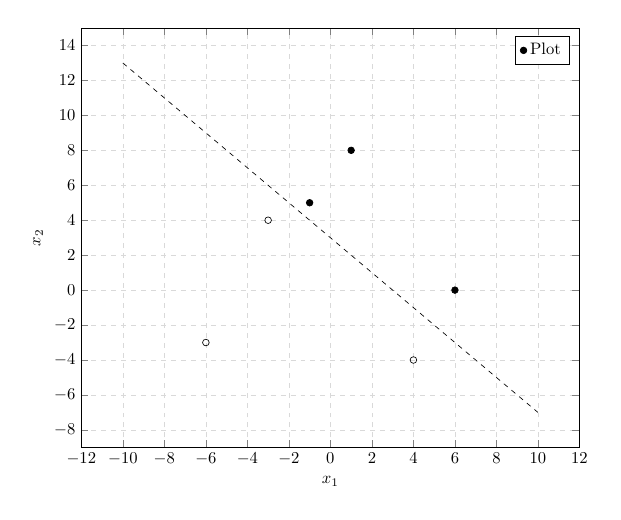
\begin{tikzpicture}[scale=.6]
		\begin{axis}[
			width=\linewidth, % Scale the plot to \linewidth
    	     	grid=major, % Display a grid
    	      	grid style={dashed,gray!30}, % Set the style
			xlabel=$x_1$,
			ylabel=$x_2$,
		    %xtick=\empty, ytick=\empty
		]
		\addplot [only marks] table {
			1 8
			6 0
			-1 5
		};
		
		\addplot [only marks, mark=o] table {
			-6 -3
			4 -4
			-3 4
		};
		\addplot [domain=-10:10, samples=2, dashed] {-x + 3};

        \legend{Plot}
      \end{axis}
	\end{tikzpicture}
	\caption{Representation of perceptron's decision separation.}\label{fig:perceptron-boundaries}
\end{figure}
As the Perceptron the goal of MLP is to approximate a function $f^{*}$ that should represents the underlying data with which the neural network is trained, e.g. a classifier where $y=f^{*}(\textbf{x})$ associates an example record $\textbf{x}$ to class $y$.\newline\newline
These models set, that include also single layered perceptron, are called \textit{feedforward} because the information flows through the input layer, that contains the data from the example \textbf{x}, through all the intermediate layers called \textbf{hidden layers} and finally to the output layer $\textbf{y}$. So all these levels are connected only with the ones next and feedback connections that fed back the network are missing. Neural networks having this exclusive characteristic are called \textbf{recurrent neural networks}.\newline\newline
To all of these layer are associated different functions, called \textbf{activation functions}, that allow the layers to produce non-linear output values. Thus, in an other perspective, a feedforward can be seen as a chain of activation functions. From this description we can see that the major difference between single-layered Perceptron and feedforward neural networks is the training strategy. In fact the design of the FFN prevents to approach the training with the same strategy used with the Perceptron because we does not have \textit{a priori} the informations regard the desired output of all the hidden layers, so we can not update the weights as we have seen in the Perceptron.
\begin{figure}[t]
	\centering
	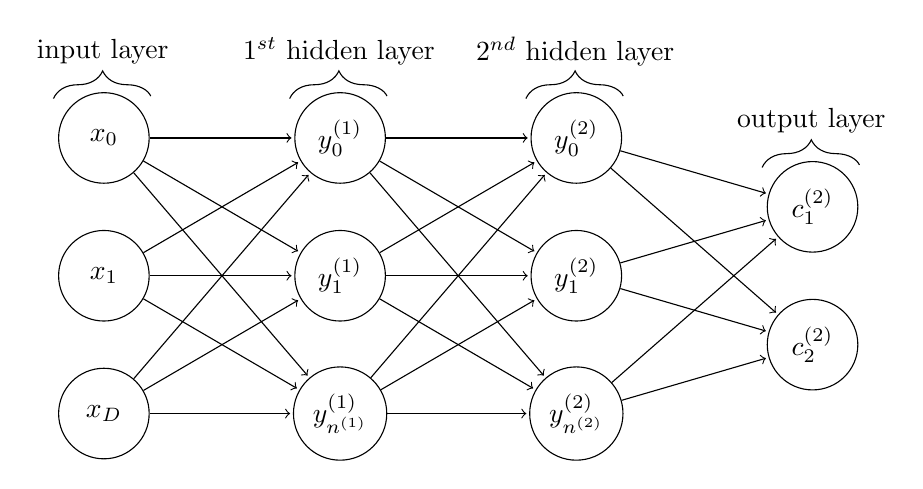
\begin{tikzpicture}[shorten >=1pt]
		\tikzstyle{unit}=[draw,shape=circle,minimum size=1.15cm]
		%\tikzstyle{hidden}=[draw,shape=circle,fill=black!25,minimum size=1.15cm]
		\tikzstyle{hidden}=[draw,shape=circle,minimum size=1.15cm]

		\node[unit](x0) at (0,3.5){$x_0$};
		\node[unit](x1) at (0,1.75){$x_1$};
		%\node at (0,1.075){\vdots};
		\node[unit](xd) at (0,0){$x_D$};

		\node[hidden](h10) at (3,3.5){$y_0^{(1)}$};
		\node[hidden](h11) at (3,1.75){$y_1^{(1)}$};
		%\node at (3,1.075){\vdots};
		\node[hidden](h1m) at (3,0){$y_{n^{(1)}}^{(1)}$};
		
		\node[hidden](hL0) at (6,3.5){$y_0^{(2)}$};
		\node[hidden](hL1) at (6,1.75){$y_1^{(2)}$};
		%\node at (6,1.075){\vdots};
		\node[hidden](hLm) at (6,0){$y_{n^{(2)}}^{(2)}$};

		\node[unit](y1) at (9,2.625){$c_1^{(2)}$};
		\node[unit](y2) at (9,00.875){$c_2^{(2)}$};
		%\node at (9,1.075){\vdots};	
		%\node[unit](yc) at (9,0){$c_C^{(2)}$};

		
		\draw[->] (x0) -- (h10);
		\draw[->] (x0) -- (h11);
		\draw[->] (x0) -- (h1m);

		\draw[->] (x1) -- (h10);
		\draw[->] (x1) -- (h11);
		\draw[->] (x1) -- (h1m);

		\draw[->] (xd) -- (h10);
		\draw[->] (xd) -- (h11);
		\draw[->] (xd) -- (h1m);

		\draw[->] (hL0) -- (y1);
		\draw[->] (hL0) -- (y2);
		%\draw[->] (hL0) -- (yc);

		\draw[->] (hL1) -- (y1);
		\draw[->] (hL1) -- (y2);
		%\draw[->] (hL1) -- (yc);

		\draw[->] (hLm) -- (y1);
		\draw[->] (hLm) -- (y2);
		%\draw[->] (hLm) -- (yc);

		\draw[->] (h10) -- (hL0);
		\draw[->] (h11) -- (hL0);
		\draw[->] (h1m) -- (hL0);
		
		\draw[->] (h10) -- (hL1);
		\draw[->] (h11) -- (hL1);
		\draw[->] (h1m) -- (hL1);
		
		\draw[->] (h10) -- (hLm);
		\draw[->] (h11) -- (hLm);
		\draw[->] (h1m) -- (hLm);
		
		\draw [decorate,decoration={brace,amplitude=10pt},xshift=-4pt,yshift=0pt] (-0.5,4) -- (0.75,4) node [black,midway,yshift=+0.6cm]{input layer};
		\draw [decorate,decoration={brace,amplitude=10pt},xshift=-4pt,yshift=0pt] (2.5,4) -- (3.75,4) node [black,midway,yshift=+0.6cm]{$1^{\text{st}}$ hidden layer};
		\draw [decorate,decoration={brace,amplitude=10pt},xshift=-4pt,yshift=0pt] (5.5,4) -- (6.75,4) node [black,midway,yshift=+0.6cm]{$2^{\text{nd}}$ hidden layer};
		\draw [decorate,decoration={brace,amplitude=10pt},xshift=-4pt,yshift=0pt] (8.5,3.125) -- (9.75,3.125) node [black,midway,yshift=+0.6cm]{output layer};
	\end{tikzpicture}
	\caption[Graph representation of feedforward neural network.]{Graph representation of feedforward neural network with $(2)$-layer, with $D$ input units and $2$ output units (class). For simplicity of representation all the labels $w_{ij}$ associated to the edges, that represent the weights/parameters of the neural networks, are omitted.}
	\label{fig:multilayer-perceptron}
\end{figure}

\subsection{Activation functions}\label{sec:activation-functions}
The activation functions are special functions that can be, in particular, differentiable. This last characteristic is mandatory if the used optimization algorithm is gradient based. These functions are used in every neurons of an ANN and define how the neurons emit their values when stimulated. The following are some activation functions with their plots:\newline\newline

\begin{tabular*}{\textwidth}{@{} l @{\extracolsep{\fill}} r @{}}
\centering
\begin{minipage}{0.475\textwidth}
	\begin{tabular}{c}
			\(\displaystyle
				\sigma(x) = x
			\) \\\\
			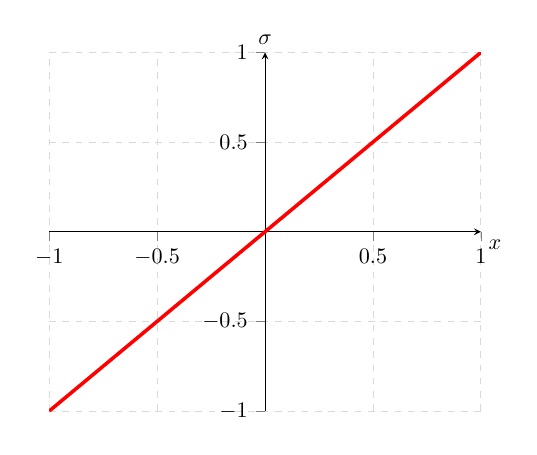
\begin{tikzpicture}[smooth,scale=0.8]
				\begin{axis}[
    					axis x line=middle,
    					axis y line=middle,
    					grid = major,
	    				grid style={dashed, gray!30},
      				xlabel=$x$,
   					ylabel=$\sigma$,
					xlabel style={below right},
					ylabel style={above},
    					tick align=outside,
	    				enlargelimits=false,	
				]
    					\addplot+[mark=none,ultra thick, red, domain=-1:1, samples=500] {x};
				\end{axis}
			\end{tikzpicture}
	\end{tabular}
	\captionof{figure}{Linear activation function.}
\end{minipage}&
\begin{minipage}{0.475\textwidth}
	\begin{tabular}{c}
			\(\displaystyle
				\sigma(x) = \begin{cases}
					0, & \textrm{for}\ x < 0 \\
					x, & \textrm{for}\ x >= 0
				\end{cases}
			\) \\
			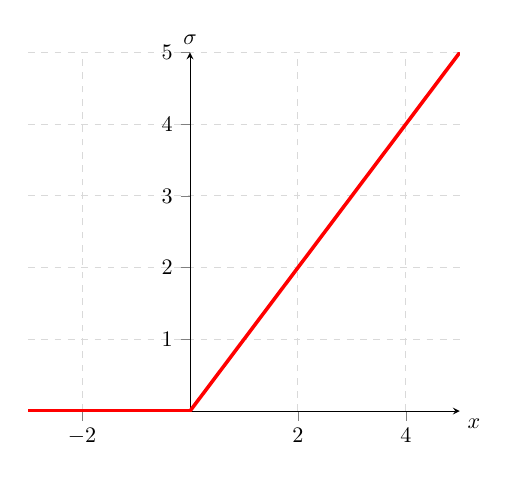
\begin{tikzpicture}[smooth,scale=.80]
				\begin{axis}[
        				axis x line=middle,
        				axis y line=middle,
        				grid = major,
        				grid style={dashed, gray!30},
        				xlabel=$x$,
        				ylabel=$\sigma$,
  					xlabel style={below right},
  					ylabel style={above},
        				tick align=outside,
        				enlargelimits=false,	
				]
        				\addplot+[mark=none,ultra thick, red, domain=-3:0, samples=500] {0};
        				\addplot+[mark=none,ultra thick, red, domain=0:5, samples=500] {x};
				\end{axis}
			\end{tikzpicture}
	\end{tabular}
	\captionof{figure}{ReLu activation function.}
	\end{minipage} \\
\begin{minipage}{0.475\textwidth}
	\begin{tabular}{c}
		\(\displaystyle
			\sigma(x) = \frac{1}{1 + e^{-x}} = \frac{e^{x}}{e^{x} + 1}
		\) \\\\
		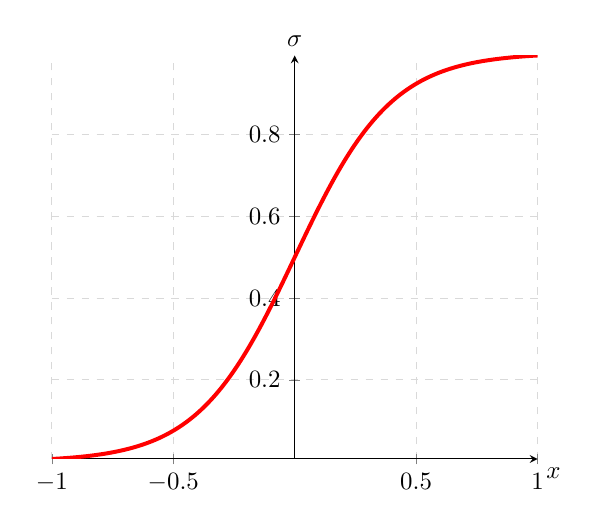
\begin{tikzpicture}[smooth,scale=.9]
			\begin{axis}[
  				axis x line=middle,
		        	axis y line=middle,
			    	grid = major,
    		    		grid style={dashed, gray!30},
			    ylabel=$\sigma$,
		    		xlabel=$x$,
  				xlabel style={below right},
	  			ylabel style={above},
			]
      			\addplot[domain=-1:1, red, ultra thick,samples=500] {1/(1+exp(-5*x))};
			\end{axis}
		\end{tikzpicture}
	\end{tabular}\captionof{figure}{Sigmoid activation function.}
\end{minipage} &
\begin{minipage}{0.475\textwidth}
	\begin{tabular}{c}
		\(\displaystyle
			\sigma(x) = \frac{e^{x} - e^{-x}}{e^{x} + e^{-x}}
		\) \\\\
		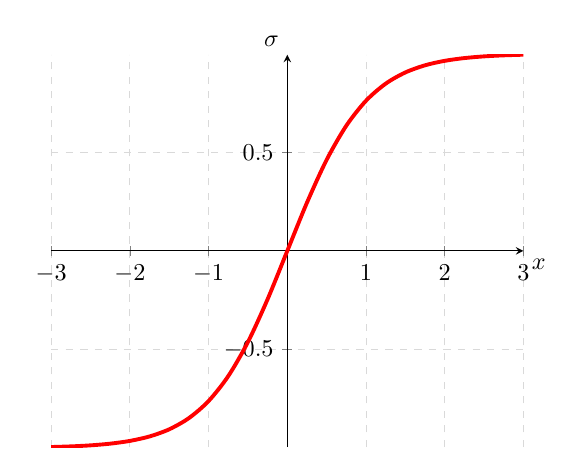
\begin{tikzpicture}[smooth,scale=.875]																	\setlength{\belowcaptionskip}{-10pt}
			\begin{axis}[
  				axis x line=middle,
			    axis y line=middle,
				grid = major,
    			    grid style={dashed, gray!30},
				ylabel=$\sigma$,
		    		xlabel=$x$,
  				xlabel style={below right},
	  			ylabel style={above left},
  				domain=-3:3
			]
    				\addplot [mark=none,draw=red,ultra thick] {tanh(\x)};
			\end{axis}
		\end{tikzpicture}
	\end{tabular}\captionof{figure}{Tanh activation function.}
\end{minipage}

\end{tabular*}
\clearpage
\section{Artificial Neural Network training} 
The training of ANN generally follows two main steps: the initialization of the weight of the connections and the re-compute of these with an iterative algorithm which is guided by the optimization of an objective function\footnote{In specific we speak of \textbf{cost} or \textbf{loss} function if the objective is to minimize this latter.}, searching for a global minimum\footnote{Obviously the global minimum is not guaranteed and this depend by the problem, the ANN design and the optimization algorithm. Often what is found is a local minimum, which not guarantee that the ANN represents the underlying data.}. The specific operations in the second step can be further split in two sub-steps: firstly the objective function is computed, then in the second step the weight of the connections are updated with some strategy/algorithm according to the objective function value. 

\begin{algorithm}
	\begin{algorithmic}[1]
		\State{Let $D = \{(\textbf{x}_i, y_i)\ |\ i  = 1, \dots, N\}$ be the set of examples.}
		\State{Let $\lambda$ a small real valued learning rate}
		\State{Initialize the weights vector with random values, $\textbf{w}^{(0)}$}
		\Repeat
			\For{ each batch of $(\textbf{x}_{i}, y_{i}) \in D$}
				\State{Compute the predicted output $\hat{y}_{i}^{(k)}$}
				\State{Compute the gradient $\delta$ for each $w_{ij}$ with backpropagation}
				\For{ each weight $w_{ij}$}
					\State{Update the weight $w_{ij}$ with some strategy using the associated $\delta$ and the learning rate $\lambda$}
				\EndFor
			\EndFor
		\Until{ Convergence is met }
	\end{algorithmic}
	\caption{Flow of a general algorithm based on the gradient for ANNs.}\label{alg:ann-training}
\end{algorithm}

\subsection{Gradient based optimization algorithms}
Once the gradients are computed according to the objective function, for example with the backpropagation technique presented in Section \ref{subsubsec:backpropagation}, they can be used to re-compute the associated parameters. To do this exist some optimization algorithms that implement gradient descent. These algorithm have as objective the research of the global minimum of the cost function with a research that, with a similitude, is similar to the descent of a bowl (that can be associated to the complete plot of the objective function) by an hypothetical ball, where the bowl bottom corresponds to the global minimum of the function.
\begin{figure}[!ht]
     \subfloat[The Gradient Descent can be seen as the descent of a bowl by a ball. The end of each arrow is a descent step of an hypothetical ball. With the red and blue are represented respectively the zones of maximum and minimum. (Yes, this figure seems more similar to the planet Saturn.)\label{subfig-1:gradient-descent-1}]{%
		\begin{tikzpicture}[samples=100,smooth, scale=.875]
			\begin{scope}
				\draw[opacity=0,fill=GDFirst,fill opacity=1] plot[domain=0:360] ({cos(\x)*sqrt(20/(sin(2*\x)+2))},{sin(\x)*sqrt(20/(sin(2*\x)+2))});
				\draw[opacity=0,fill=GDSecond,fill opacity=1] plot[domain=0:360] ({cos(\x)*sqrt(16/(sin(2*\x)+2))},{sin(\x)*sqrt(16/(sin(2*\x)+2))});
				\draw[opacity=0,fill=GDThird,fill opacity=1] plot[domain=0:360] ({cos(\x)*sqrt(12/(sin(2*\x)+2))},{sin(\x)*sqrt(12/(sin(2*\x)+2))});
				\draw[opacity=0,fill=GDFourth,fill opacity=1] plot[domain=0:360] ({cos(\x)*sqrt(8/(sin(2*\x)+2))},{sin(\x)*sqrt(8/(sin(2*\x)+2))});
				\draw[opacity=0,fill=GDFiveth,fill opacity=1] plot[domain=0:360] ({cos(\x)*sqrt(4/(sin(2*\x)+2))},{sin(\x)*sqrt(4/(sin(2*\x)+2))});
				\draw[opacity=0,fill=GDSixth,fill opacity=1] plot[domain=0:360] ({cos(\x)*sqrt(1/(sin(2*\x)+2))},{sin(\x)*sqrt(1/(sin(2*\x)+2))});
				\draw[opacity=0,fill=GDSeventh,fill opacity=1] plot[domain=0:360] ({cos(\x)*sqrt(0.0625/(sin(2*\x)+2))},{sin(\x)*sqrt(0.0625/(sin(2*\x)+2))});
			
				\draw[->,blue,ultra thick] (-2,3.65) to (-1.93,3);
				\draw[->,blue,ultra thick] (-1.93,3) to (-1.75,2.4);
				\draw[->,blue,ultra thick] (-1.75,2.4) to (-1.5,1.8);
				\draw[->,blue,ultra thick] (-1.5,1.8) to (-1.15,1.3);
			
				%\node at (-1.4,3.8){\scriptsize $w[0]$};
				%\node at (-1.2,3.2){\scriptsize $w[1]$};
				%\node at (-1.05,2.6){\scriptsize $w[2]$};
				%\node at (-0.8,2){\scriptsize $w[3]$};
				%\node at (-0.6,1.4){\scriptsize $w[4]$};
			\end{scope}
		\end{tikzpicture}     
	}
     \hfill
     \subfloat[Second example plot of gradient descent. As we can see is not certain that the global maximum can be reached in the descent. \label{subfig-2:gradient-descent-2}]
     {%	
     \begin{tikzpicture}[smooth,scale=.875]
			\begin{axis}[
  				axis x line=center,
  				axis y line=center,
  				xlabel={$x1$},
  				ylabel={$x2$},
  				xlabel style={below right},
  				ylabel style={above left},	
			    xmin=0, xmax=1,
			    ymin=0, ymax=1,
				legend pos=north east  			
			]
  				\addplot[mark=none, black] table{data/gradient-descent-data.txt};
  				\addlegendentry{Cost}

  				
  				\addplot+[mark=o, red] coordinates {
    					(0.335,   0.38)
  				};				
  				\addlegendentry{Local minimum}


  				\addplot+[mark=o, blue] coordinates {
    					(0.95,   0.1)
  				};  				
  				\addlegendentry{Global minimum}

			\end{axis}
	\end{tikzpicture}
	}
	\label{fig:dummy}
\end{figure}
This research of a better parameters configuration not only works with the discovered delta, but also with a parameter $\lambda$ called learning rate, that must be small for a better research. Hence, to all weights are not associated only $\delta$ but 
\begin{equation}
	\Delta{w_{ij}} = -\lambda\frac{\partial{E}}{\partial{w_{ij}}}
\end{equation}\label{eq:delta-learning-rate}

\subsubsection*{Stochastic Gradient Descent (SGD)}
Using the equation \ref{eq:delta-learning-rate} the parameters are updated as follows
\begin{equation}
	w_{ij}^{(t + 1)} = w_{ij}^{(t)} - \lambda\frac{\partial{E}}{\partial{w_{ij}}} 
\end{equation}

\subsubsection*{Adaptive Moment (ADAM)}
Let $\beta_1$ and $\beta_2$ exponential decay rates used for the momentum estimates, $m_0$ the $1^{st}$ moment vector, $v_0$ the $2^{nd}$ moment vector and $\epsilon$ a small real valued scalar we have 
\begin{align}
	m_{ij}^{(t)} &= \beta_1m_{ij}^{(t-1)} + (1 - \beta_1)\delta_{ij}^{(t)} \\
	v_{ij}^{(t)} &= \beta_2v_{ij}^{(t-1)} + (1 - \beta_2)\delta_{ij}^{2,  (t)} \\
	\hat{m}_{ij}^{(t)} &= \frac{m_{ij}^{(t)}}{1 - \beta_{1}} \\
	\hat{v}_{ij}^{(t)} &= \frac{v_{ij}^{(t)}}{1 - \beta_{2}} \\
	w_{ij}^{(t)} &= w_{ij}^{(t)} - \lambda\frac{\hat{m}_{ij}^{(t)}}{\sqrt{\hat{v}_{ij}^{(t)}} + \epsilon}
\end{align}
\paragraph{Momentum}
The technique of momentum \cite{POLYAK19641} takes inspiration to physical environment. It is used  to accelerate learning\footnote{In Stochastic Gradient, so also in ADAM, it is used to resolve the variance of the gradient.}, specially in case of high curvature, small and noisy gradients. Formally, the momentum is represented by a vector \textbf{v} that plays the role of velocity, i.e. the direction and speed of parameters moving through the parameters space. It is used in learning as a force to avoid that the gradients move too freely\footnote{In this case, with a physical similitude, we can see the gradients as a hockey puck sliding on a frictionless icy surface.}, conditioning too much the descent. In other words, the momentum helps the descent to move in the direction of most weight gradients push. In ADAM there are two momentum vectors, respectively the mean and the uncentered variance of the gradients. 

\subsubsection{Backpropagation}\label{subsubsec:backpropagation}
Backpropagation is an algorithm introduced in \cite{RUM:1986} used to optimize the weights of a neural network. For a batch of data it computes the contribution in the error of each neurons with respect to an objective function, which should capture the differences between the expected output, i.e. the $y$, and the generated output, i.e. the $\hat{y}$, transforming those in a real value. An example of objective function is the Total Sum of Squared errors:
\begin{equation}
	TSS = \frac{1}{2}\sum\limits_{i=1}^{N}(y_i - \hat{y}_{i})^{2}
\end{equation}\label{eq:tss}
The backpropagation is divided into two phases, the forward and the backward propagation.

\paragraph{Forward propagation}
Intuitively, in the forward propagation pass the network is "forward executed", i.e. starting from a batch of example, the computations for all the layers are executed up to the output layer in a forward manner. Formally, let $D = \{(\textbf{x}_{i}, y_{i})\ |\ i=1,\ \dots ,\ N \}$ the set of examples, $L = \{(l^{(j)}_{h}, b^{(j)}_{h})\ |\ j = 1,\ \dots,\ M,\ $h is the neurons of the layer$\}$ the set of FNN hidden layers and $A = \{\alpha^{(i)}\ |\ i = 1,\ \dots,\ M\}$. Then selected the sample $(\textbf{x}_i, y_i)$ the parameters, i.e. the weights, for the first level are computed in this way
\begin{equation}
	a^{(1)} = \alpha^{(1)}(\sum\limits_{i=1}^{|\textbf{x}|}x_{i}l_{h}^{(1)} + b^{(1)})
\end{equation}
where $\alpha^{(1)}$ is the activation function of the first layer.\\
Subsequently, as state previously, the computation continue forward for all the other hidden layers as follows
\begin{equation}
	a^{(j)} = \alpha^{(j)}(\sum\limits_{n \in a^{(j - 1)}}a^{(j - 1)}_{n}h^{(j)}_{h} + b^{(j)})
\end{equation}
where the $h^{(j - 1)}$ are the computed weights of the previous layer of the layer $h^{(j)}$, up to the output layer where we have
\begin{equation}
	\hat{y} = \alpha^{(M)}(\sum\limits_{n \in a^{(M - 1)}}a^{(M - 1)}_{n}o + b^{(M)})	
\end{equation}
where $\hat{y}$ is the neural networks output that will be used in the backward propagation step and $o = h^{M}_{h = C}$.

\paragraph{Backward propagation}
Once the objective function is computed the backward propagation can be executed. A strictly requirement is that all the activation functions and the objective function must be differentiable, because it uses the technique of Chain Rule of calculus which, basically, computes the derivatives of functions formed by composing other functions whose derivatives are known.\newline\newline
This make it possible to calculate the error for each node starting from the output layer in a backward mode, i.e. for each layers, starting from the output layer, it is calculated the $\delta$ for all the weights which is contribute to the ANN errors, named also gradient. Make it clearer with an example where we calculate the gradient $\delta$ for a generic parameter of the FNN, so let \textbf{TSS} the loss function in \ref{eq:tss} and $w_{ij}$ a parameter\footnote{The connection between two neurons.} for the neuron $j^{th}$ of $l$ arriving from the $i^{th}$ neuron of the previous layer $l-1$. Starting examining the partial derivative of error with respect to the parameter $w_{ij}$ applying the chain rule
\begin{equation}
	\frac{\partial{TSS}}{\partial{w_{ij}}} = \frac{\partial{TSS}}{\partial{neur_j}}\frac{\partial{neur_j}}{\partial{\alpha_j}}\frac{\partial{\alpha_j}}{\partial{w_{ij}}}
\end{equation}\label{eq:partial-derivative-w_ij}
Now let's examine the parts of this partial derivative, we have for the first term
\begin{equation}
	\frac{\partial{TSS}}{\partial{neur_j}} = \frac{\partial{TSS}}{\partial{y}} = \frac{\partial{}}{\partial{y}}\frac{1}{2}(t - y)^2 = y - t
\end{equation}\label{eq:partial-derivative-output-layer}
if the $\textrm{neur}_j = y$, i.e. we are in the output layer, otherwise we must use another way if we are in an other layer. So consider all the neurons $N_i = \{u, v, \dots, w\}$ of the $i-th$ layer that receive an input from the neuron $\textrm{neur}_j$ of the previous layer, then we have a recursive expression
\begin{equation}
	\frac{\partial{TSS}}{\partial{neur_i}} = \sum\limits_{j \in N_i}\Bigg(\frac{\partial{TSS}}{\partial\alpha_j}\frac{\partial{\alpha_j}}{\partial{neur_i}}\Bigg) = \sum\limits_{j \in N_i}\Bigg(\frac{\partial{TSS}}{\partial{neur_j}}\frac{\partial{neur_j}}{\partial{\alpha_j}}w_{ij}\Bigg)
\end{equation}\label{eq:partial-derivative-inner-layer}
Then examine the second term and we have
\begin{equation}
	\frac{\partial{neur_j}}{\partial{\alpha_j}} = \frac{\partial{}}{\partial{\alpha_j}}\phi(\alpha_j)
\end{equation}
that as we can observe it's only the derivative of the neuron with respect to the activation function $\alpha_j$ associated to the level.\newline\newline
Finally observe the third term of \ref{eq:partial-derivative-w_ij}
\begin{equation}
	\frac{\partial{\alpha_j}}{\partial{w_{ij}}} = \frac{\partial{}}{\partial{w_{ij}}}\Bigg(\sum\limits_{k=1}^n w_{kj}neur_k\Bigg) = \frac{\partial{}}{\partial{w_{ij}}}w_{ij}neur_i = neur_i
\end{equation}
observing that $neur_i = x_i$, if the $l_j$ is the first layer after the input layer.\newline\newline
So putting all together we have 
\begin{equation}
	\frac{\partial{TSS}}{\partial{w_{ij}}} = neur_i\delta_j
\end{equation}
where, considering the two case in \ref{eq:partial-derivative-output-layer} and \ref{eq:partial-derivative-inner-layer}, we have
\begin{equation}
	\delta_j = \frac{\partial{TSS}}{\partial{n_j}}\frac{\partial{n_j}}{\partial{\alpha_j}} = \left.
	\begin{cases}
		(n_j - \hat{y}_j)n_j(1 - n_j),\textrm{ if } n_j \textrm{ is an output neuron} \\
(\sum\limits_{r	\in N_i}\delta_{j}w_{jr})n_{j}(1 - n_{j}), \textrm{ if }n_j\textrm{ is a inner neuron}
	\end{cases}\right.
\end{equation}

\subsection{Alternatives to Gradient Descent}
Although the technique of Gradient Descent is largely used in Machine Learning for the optimization of Neural Networks, is not the unique approach to this problem. An alternative can be found in the family of Evolutionary Computation. In particular in Evolutionary Algorithms (EAs); they are a class of algorithms inspired by mechanisms of the biological evolution, used in Artificial Intelligence and Machine Learning for the research of a global optimum in a problem, i.e. a solution. This research is made evolving a set of candidates named individuals, with methods similar to which can found in Nature like reproduction, mutation, recombination and evolution. As pointed out in literature \cite{Ilonen2003DifferentialET, Morse2016SimpleEO}, also the EAs have been successfully used for the search and optimization of small feedforward neural networks. What is still unclear is how can be used and what results can be obtained with this algorithms in much more deep and greater ANNs, like NRAM.